\documentclass[10pt, aspectratio=169]{beamer}
% Shared setup for every day of the course.
\usetheme[progressbar=frametitle, numbering=fraction, block=fill]{metropolis}
\usepackage[T1]{fontenc}
\usepackage[utf8]{inputenc}
\usepackage{lmodern}
\usepackage{amsmath, amssymb, bm, booktabs, graphicx, xcolor}
\usepackage{tikz}
\usetikzlibrary{arrows.meta, positioning, calc, shapes.geometric}

\graphicspath{{figures/}}

% --- colours -------------------------------------------------------------------------------------
\definecolor{accent}{HTML}{C0392B}
\definecolor{cool}{HTML}{2E6DB4}
\definecolor{muted}{HTML}{7A7A7A}
\definecolor{good}{HTML}{2E8B57}
\setbeamercolor{alerted text}{fg=accent}
\setbeamercolor{example text}{fg=cool}

% --- notation (follows the thesis' notation chapter) ---------------------------------------------
\newcommand{\given}{\,|\,}
\newcommand{\E}{\mathbb{E}}
\newcommand{\KL}[2]{D_{\mathrm{KL}}\!\left[#1\,\middle\|\,#2\right]}
\newcommand{\N}{\mathcal{N}}
\newcommand{\Hess}{\mathcal{H}}
\newcommand{\nats}{\,\text{nats}}
\DeclareMathOperator*{\argmin}{arg\,min}

% --- course devices ------------------------------------------------------------------------------
% \src{...}: where a claim or number comes from (thesis file and line, or a post-thesis note).
\newcommand{\src}[1]{\par\vfill\hfill{\scriptsize\color{muted}source: #1}}
% \wip: marks a post-thesis result.
\newcommand{\wip}{{\scriptsize\color{white}\colorbox{accent}{\,work in progress\,}}}
% \lesson{...}: the one sentence a frame exists to say.
\newcommand{\lesson}[1]{\begin{alertblock}{}\centering #1\end{alertblock}}
% a measurement story
\newenvironment{measured}[1]{\begin{exampleblock}{Measured: #1}}{\end{exampleblock}}

\author{Course built on the doctoral thesis of No\'e Zapata}
\institute{Montevideo, 30 November -- 4 December 2026}

% \cyclemap{n}: the course's five-stage cycle, stage n highlighted (1 room ... 5 memory).
\newcommand{\cyclemap}[1]{%
  \begin{tikzpicture}[
      st/.style={draw=muted, thick, rounded corners=3pt, fill=white, align=center,
                 minimum width=2.5cm, minimum height=0.8cm, font=\scriptsize, text=muted},
      on/.style={draw=accent, very thick, fill=accent!10, text=black, font=\scriptsize\bfseries},
      arr/.style={-{Stealth[length=2mm]}, thick, color=muted},
      s1/.style={}, s2/.style={}, s3/.style={}, s4/.style={}, s5/.style={}, s#1/.style={on}]
    \node[st, s1] (c1) at (90:1.9)   {estimate the room};
    \node[st, s2] (c2) at (18:2.6)   {localise; learn\\the body};
    \node[st, s3] (c3) at (-54:2.2)  {concepts fill\\the room};
    \node[st, s4] (c4) at (-126:2.2) {cross the door};
    \node[st, s5] (c5) at (162:2.6)  {new room;\\memory};
    \draw[arr] (c1) to[bend left=15] (c2); \draw[arr] (c2) to[bend left=15] (c3);
    \draw[arr] (c3) to[bend left=15] (c4); \draw[arr] (c4) to[bend left=15] (c5);
    \draw[arr] (c5) to[bend left=15] (c1);
  \end{tikzpicture}}


\title{A robot that acts to know}
\subtitle{Day 1 --- The challenge, and free energy}
\date{Monday 30 November}

\begin{document}

\maketitle

% =================================================================================================
\section{The challenge}
% =================================================================================================

\begin{frame}{A robot is put down in an apartment it has never seen}
  \centering
  \vspace{1em}
  {\color{muted}\fbox{\parbox[c][0.55\textheight][c]{0.8\textwidth}{\centering
    \Large [ video: the full cycle, Webots / real apartment ]\\[0.5em]
    \normalsize room estimated $\rightarrow$ localised $\rightarrow$ objects appear
    $\rightarrow$ door crossed $\rightarrow$ second room}}}
  \vspace{1em}

  Watch for one thing: \alert{nothing in this video was programmed as a sequence of steps.}
\end{frame}

\begin{frame}{The cycle we will build this week}
  \centering
  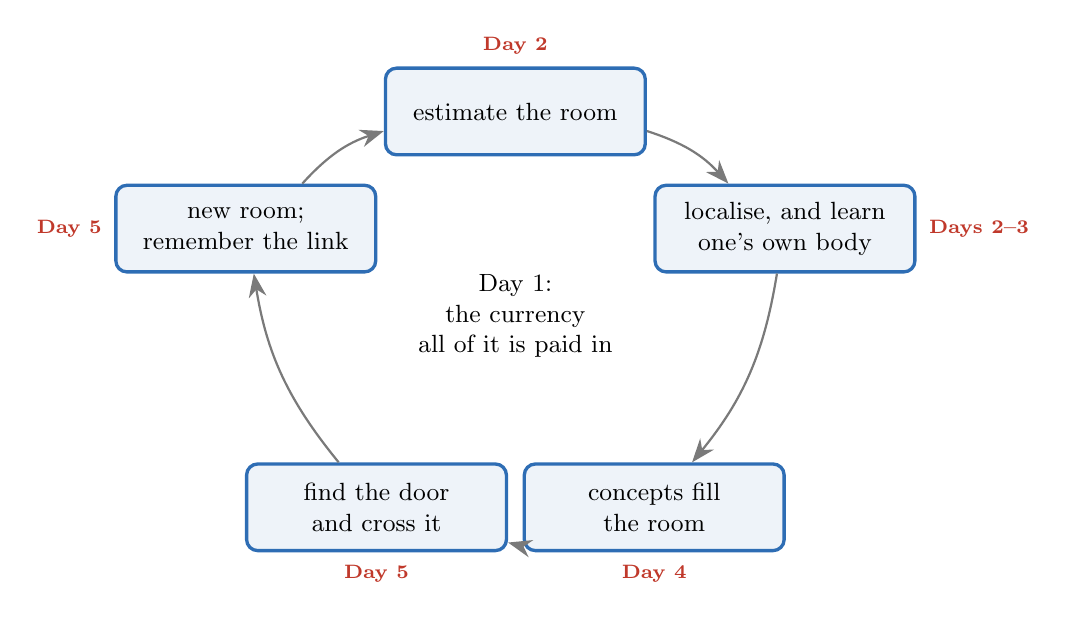
\begin{tikzpicture}[
      stage/.style={draw=cool, very thick, rounded corners=4pt, fill=cool!8, align=center,
                    minimum width=3.3cm, minimum height=1.1cm, font=\small},
      day/.style={font=\scriptsize\bfseries, text=accent},
      arr/.style={-{Stealth[length=3mm]}, thick, color=muted}]
    \node[stage] (room) at (90:2.6)   {estimate the room};
    \node[stage] (loc)  at (18:3.6)   {localise, and learn\\one's own body};
    \node[stage] (obj)  at (-54:3.0)  {concepts fill\\the room};
    \node[stage] (door) at (-126:3.0) {find the door\\and cross it};
    \node[stage] (mem)  at (162:3.6)  {new room;\\remember the link};
    \draw[arr] (room) to[bend left=15] (loc);
    \draw[arr] (loc)  to[bend left=15] (obj);
    \draw[arr] (obj)  to[bend left=15] (door);
    \draw[arr] (door) to[bend left=15] (mem);
    \draw[arr] (mem)  to[bend left=15] (room);
    \node[day, above=1pt of room] {Day 2};
    \node[day, right=1pt of loc]  {Days 2--3};
    \node[day, below=1pt of obj]  {Day 4};
    \node[day, below=1pt of door] {Day 5};
    \node[day, left=1pt of mem]   {Day 5};
    \node[align=center, font=\small] at (0,0) {Day 1:\\the currency\\all of it is paid in};
  \end{tikzpicture}
\end{frame}

\begin{frame}{Every stage is a belief}
  \footnotesize
  \begin{tabular}{@{}l l l c@{}}
    \toprule
    stage & what is unknown (latent) & what supplies the evidence & day \\
    \midrule
    estimate the room   & walls, corners, the polygon            & LiDAR returns                     & 2 \\
    localise            & the robot's pose in that room          & LiDAR against the believed room   & 2 \\
    learn the body      & wheel scale, gyro bias, sensor mounts  & the localiser's corrections       & 3 \\
    concepts            & which objects exist, where, what shape & camera masks, LiDAR               & 4 \\
    door                & where it is, whether it is open        & the room's boundary, free space   & 5 \\
    new room + memory   & a second polygon; how rooms connect    & all of the above, again           & 5 \\
    \bottomrule
  \end{tabular}

  \vspace{1.2em}
  One generative model over all of it, and \alert{one} quantity that every stage minimises:
  perception lowers it by changing beliefs, action by changing the data.
\end{frame}

\begin{frame}{The toy version you will build, one stage a day}
  \centering
  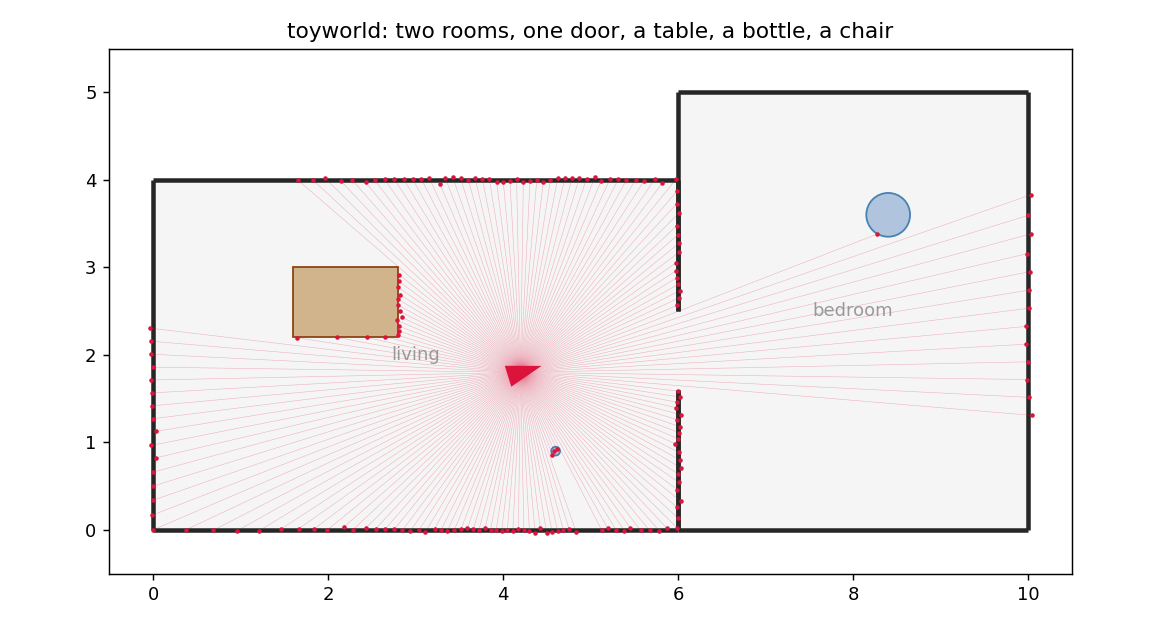
\includegraphics[width=0.78\textwidth]{toyworld.png}

  \small Two rooms, one door, three objects, a LiDAR, and a robot whose wheels lie a little.
  Pure \texttt{numpy}; it runs on your laptop.
\end{frame}

\begin{frame}{How this course is built}
  \begin{columns}[T]
    \begin{column}{0.48\textwidth}
      Each session runs through three steps:
      \begin{enumerate}
        \item the \textbf{theory}, derived rather than asserted;
        \item the \textbf{code}, one stage of the cycle, in the lab;
        \item the \textbf{measurements} that showed when the equations were wrong.
      \end{enumerate}
      \vspace{0.5em}
      The third step is not optional. Most of what the thesis learned, it learned there.
    \end{column}
    \begin{column}{0.48\textwidth}
      \begin{block}{The thread through all five days}
        Averaging removes \alert{independent} error.\\
        It does not remove \alert{shared} error.
      \end{block}
      \small
      You will meet it as:
      \begin{itemize}
        \item the common-mode ceiling;
        \item a prior re-centred on its own estimate;
        \item a fused precision better than its best member;
        \item a metric that scores what the robot never saw.
      \end{itemize}
    \end{column}
  \end{columns}
\end{frame}

% =================================================================================================
\section{Inference behind a sensory boundary}
% =================================================================================================

\begin{frame}{The agent never sees the state}
  \begin{columns}[c]
    \begin{column}{0.45\textwidth}
      \centering
      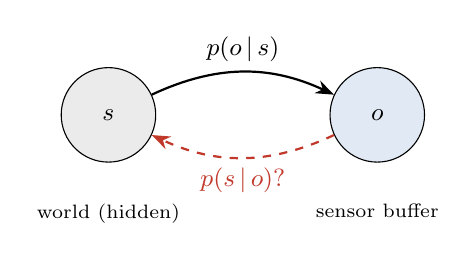
\begin{tikzpicture}[node distance=1.6cm, every node/.style={font=\small}]
        \node[draw, circle, minimum size=1.2cm, fill=muted!15] (s) {$s$};
        \node[draw, circle, minimum size=1.2cm, right=2.2cm of s, fill=cool!15] (o) {$o$};
        \draw[-{Stealth}, thick] (s) to[bend left=25] node[above] {$p(o\given s)$} (o);
        \draw[-{Stealth}, thick, accent, dashed] (o) to[bend left=25] node[below] {$p(s\given o)$?} (s);
        \node[below=0.4cm of s, align=center, font=\scriptsize] {world (hidden)};
        \node[below=0.4cm of o, align=center, font=\scriptsize] {sensor buffer};
      \end{tikzpicture}
    \end{column}
    \begin{column}{0.52\textwidth}
      The \textbf{generative model}:
      \[ p(s,o) = p(o\given s)\,p(s) \]
      \begin{itemize}\small
        \item $p(o\given s)$ is the agent's theory of its own sensor: which LiDAR returns a robot at
              this pose, in this room, would produce.
        \item $p(s)$ is what it brought with it: plausible room shapes, typical table sizes.
      \end{itemize}
      Inference runs the arrow backwards:
      \[ p(s\given o) = \frac{p(o\given s)\,p(s)}{p(o)} \]
    \end{column}
  \end{columns}
  \src{active\_inference.tex l.181--212}
\end{frame}

\begin{frame}{Where exact inference dies}
  \[ p(o) = \int p(o\given s)\,p(s)\,\mathrm{d}s \]
  \begin{itemize}
    \item The probability of \emph{this scan} under \emph{every} room and furniture configuration
          the robot considers possible, each weighted by how likely it is.
    \item No closed form and no feasible quadrature. This is not a quirk of one sensor: it is the
          generic situation.
    \item Every practical method from here on is a way of \alert{not computing it}.
  \end{itemize}
  \vspace{0.8em}
  \begin{block}{A word about ``state''}
    $s$ is a latent variable of the \emph{agent's model}, not the physical truth, which is never
    accessible. That distinction is what gives the question ``is this belief wrong?'' its meaning.
  \end{block}
  \src{active\_inference.tex l.200--220}
\end{frame}

% =================================================================================================
\section{Variational free energy}
% =================================================================================================

\begin{frame}{Do not compute the posterior; approximate it}
  Choose a tractable family, and a member $q(s)$ of it (the \textbf{belief}). Move it towards
  the true posterior, measuring closeness by
  \[ \KL{q(s)}{p(s\given o)} = \int q(s) \ln\frac{q(s)}{p(s\given o)}\,\mathrm{d}s \;\ge 0 . \]
  \pause
  \alert{Problem:} it contains $p(s\given o)$, the very thing we cannot have.

  \pause
  \vspace{0.5em}
  Substitute Bayes' rule and separate out the part that does not depend on $q$:
  \[
    \KL{q}{p(s\given o)} = \underbrace{\int q(s)\ln\frac{q(s)}{p(o,s)}\,\mathrm{d}s}_{F[q,o]} \;+\; \ln p(o)
  \]
  $F$ needs only the belief and the joint $p(o\given s)p(s)$ the agent already wrote down.
  \src{active\_inference.tex l.222--250}
\end{frame}

\begin{frame}{The identity the framework rests on}
  \[ \boxed{\; F[q,o] = \KL{q(s)}{p(s\given o)} - \ln p(o) \;} \]
  \begin{columns}[T]
    \begin{column}{0.48\textwidth}
      \begin{block}{Reading 1: same minimiser}
        $\ln p(o)$ does not depend on $q$. Minimising the computable $F$ minimises the
        uncomputable divergence.
      \end{block}
    \end{column}
    \begin{column}{0.48\textwidth}
      \begin{block}{Reading 2: a bound on surprise}
        $\mathrm{KL}\ge 0$, so $F \ge -\ln p(o)$. Lowering $F$ makes the belief better \emph{and}
        the data less surprising under the agent's own model.
      \end{block}
    \end{column}
  \end{columns}
  \vspace{0.8em}
  If you know machine learning: $-F$ is the \textbf{ELBO}. Maximising the ELBO and minimising free
  energy are the same operation.
  \src{active\_inference.tex l.252--268}
\end{frame}

\begin{frame}{Complexity minus accuracy}
  \[
    F[q,o] = \underbrace{\KL{q(s)}{p(s)}}_{\text{complexity}}
             \;-\; \underbrace{\E_q\!\left[\ln p(o\given s)\right]}_{\text{accuracy}}
  \]
  \begin{itemize}
    \item \textbf{Accuracy} rewards beliefs under which the data are likely. On its own, it would
          adopt any explanation that fits the current scan.
    \item \textbf{Complexity} charges for the distance travelled from the prior: Occam's razor,
          written as a divergence.
    \item Free energy picks the belief that buys the most accuracy for the least departure from
          what was already believed.
  \end{itemize}
  \lesson{One trade, stated once, in nats, for every quantity the agent believes.}
  \src{active\_inference.tex l.288--308}
\end{frame}

\begin{frame}{Worked example: the Kalman update is free-energy minimisation}
  \small
  Take the prior $s\sim\N(m,p)$, an observation $y\sim\N(s,r)$, and the belief $q=\N(\mu,\Sigma)$.
  Every term is a Gaussian expectation:
  \[
    F(\mu,\Sigma) = \frac{(\mu-m)^2+\Sigma}{2p} + \frac{(y-\mu)^2+\Sigma}{2r} - \tfrac12\ln\Sigma + \text{const}
  \]
  \pause
  \begin{columns}[T]
    \begin{column}{0.48\textwidth}
      $\partial F/\partial\mu = 0$:
      \[ \mu = \frac{m/p + y/r}{1/p + 1/r} \]
      the precision-weighted mean.
    \end{column}
    \begin{column}{0.48\textwidth}
      $\partial F/\partial\Sigma = 0$:
      \[ \frac1\Sigma = \frac1p + \frac1r \]
      precisions add.
    \end{column}
  \end{columns}
  \vspace{0.5em}
  \pause
  The two halves come from different terms. The \emph{mean} comes from the prediction errors; the
  \emph{variance} comes from the curvature of $F$ balanced against the entropy
  $-\tfrac12\ln\Sigma$. Regularised least squares is the same trade with a flat prior.
\end{frame}

\begin{frame}{A choice, marked as a choice}
  \begin{itemize}
    \item Closeness was measured with $\mathrm{KL}$. Nothing forced that: it is the $\alpha\to1$
          member of the Rényi family, and the bound survives the substitution.
    \item The order $\alpha$ controls the \emph{character} of the error: does the belief err
          towards too broad, or towards too confident?
    \item On this robot, that is not a statistical nicety. A covariance is \alert{spent}: on
          deciding where to look next, and on how far a measurement may move a belief.
  \end{itemize}
  \vspace{0.5em}
  The thesis keeps $\alpha\to1$ throughout. Making $\alpha$ itself a latent variable is open
  future work.
  \src{active\_inference.tex l.270--286; future\_work.tex l.22}
\end{frame}

% =================================================================================================
\section{The Laplace approximation}
% =================================================================================================

\begin{frame}{Gaussian beliefs: the form everything later takes}
  Take $q(s)=\N(\mu,\Sigma)$ and expand around the mode:
  \[
    F \approx -\ln p(o,\mu) + \tfrac12\operatorname{tr}(\Hess\Sigma) - \tfrac12\ln|\Sigma| - \tfrac n2\ln(2\pi e),
    \qquad \Hess = -\nabla^2_s \ln p(o,s)\big|_{\mu}
  \]
  \begin{itemize}
    \item The \textbf{mean} moves to the mode of the joint: a nonlinear least-squares problem
          (Gauss--Newton).
    \item The \textbf{covariance} is pulled two ways: the curvature term shrinks it, the entropy
          term widens it. Setting $\partial F/\partial\Sigma=0$:
  \end{itemize}
  \[ \boxed{\;\Sigma = \Hess^{-1}\;} \]
  \lesson{The uncertainty comes as a by-product of fitting, at no extra modelling cost.}
  \src{active\_inference.tex l.310--333}
\end{frame}

\begin{frame}{Gauss--Newton, in one line}
  For whitened residuals $r(s)$ with noise covariance $R$, and a Gaussian prior $\N(m,P)$:
  \[
    -\ln p(o,s) = \tfrac12 r^\top R^{-1} r + \tfrac12 (s-m)^\top P^{-1}(s-m) + \text{const},
  \]
  \[
    \Hess \approx J^\top R^{-1} J + P^{-1}, \qquad
    \Delta s = -\Hess^{-1}\big(J^\top R^{-1} r + P^{-1}(s-m)\big).
  \]
  \begin{itemize}
    \item Iterate to convergence. The final $\Hess^{-1}$ \emph{is} the belief's covariance.
    \item In the lab, \texttt{laplace(residual, x0, sigma, prior=...)} does exactly this. It also
          returns the Laplace free energy
          $F \approx -\ln p(o,\mu) + \tfrac12\ln|\Hess| - \tfrac n2\ln 2\pi$,
          which you will use to compare models.
  \end{itemize}
\end{frame}

\begin{frame}{Example: one wall as a belief}
  \begin{columns}[c]
    \begin{column}{0.55\textwidth}
      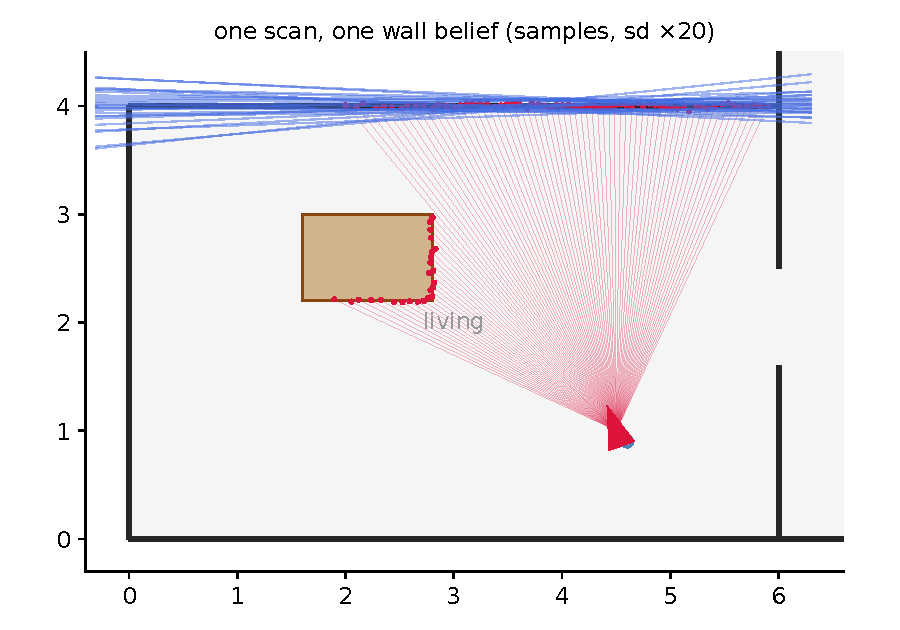
\includegraphics[width=\textwidth]{d1_wall_belief.pdf}
    \end{column}
    \begin{column}{0.43\textwidth}
      \small
      A line with normal $n(\alpha)$ at distance $d$:
      \[ r_i = \cos\alpha\,x_i + \sin\alpha\,y_i - d \]
      \[ \frac{\partial r_i}{\partial(\alpha,d)} = \big[\,-\sin\alpha\,x_i + \cos\alpha\,y_i,\; -1\,\big] \]
      \begin{itemize}
        \item The first column is a \textbf{lever arm}. Points far apart along the wall pin the
              angle.
        \item $\alpha$ and $d$ come out correlated ($\rho\approx-0.97$), because $d$ is measured
              from an origin the points are far away from.
      \end{itemize}
    \end{column}
  \end{columns}
\end{frame}

\begin{frame}{Is the covariance honest?}
  \begin{columns}[c]
    \begin{column}{0.45\textwidth}
      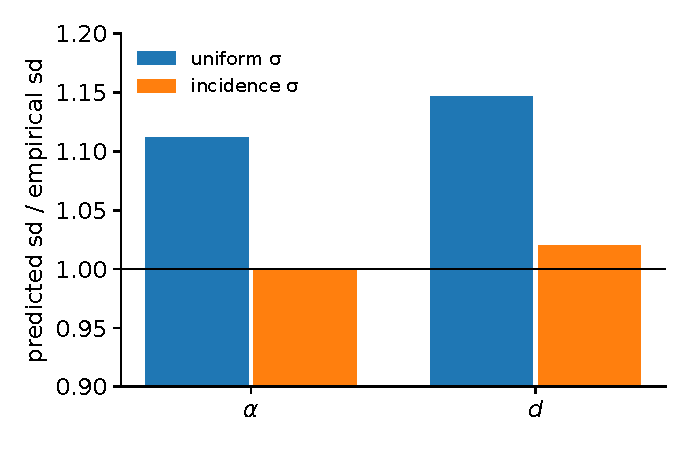
\includegraphics[width=\textwidth]{d1_honesty.pdf}
    \end{column}
    \begin{column}{0.53\textwidth}
      \small
      $\Sigma=\Hess^{-1}$ is a \emph{claim} about how far the fit would move on a re-scan.
      Test it with 400 scans from one pose:
      \begin{itemize}
        \item uniform $\sigma$: about 10\% too pessimistic, and it does not average away;
        \item the noise is along the \emph{beam}, the residual along the wall's \emph{normal}:
              $\sigma_i=\sigma\,|u_i^\top n|$;
        \item with that likelihood: within a few per cent.
      \end{itemize}
    \end{column}
  \end{columns}
  \lesson{A Laplace covariance is exactly as honest as the likelihood you wrote.}
  \src{lab 1, exercises 3--4; the real localiser's incidence weight: room\_concept.tex l.232}
\end{frame}

\begin{frame}{Free energy compares models: the price of a parameter}
  \begin{columns}[c]
    \begin{column}{0.45\textwidth}
      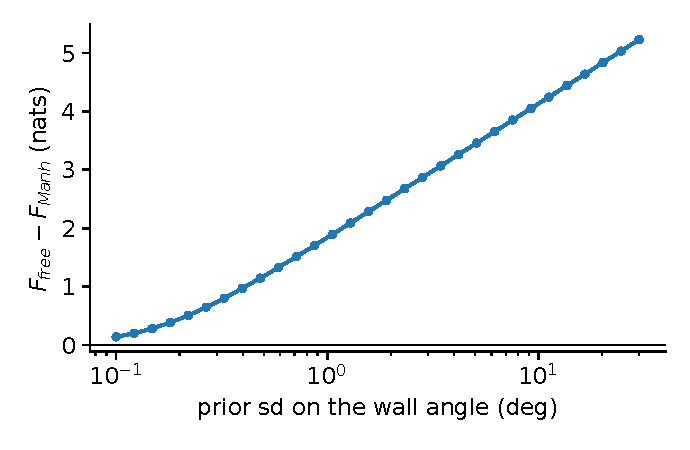
\includegraphics[width=\textwidth]{d1_occam.pdf}
    \end{column}
    \begin{column}{0.53\textwidth}
      \small
      Two models of the same wall:
      \begin{itemize}
        \item \textbf{Manhattan}: the angle is fixed at $90^\circ$; one parameter, $d$.
        \item \textbf{free}: $\alpha\sim\N(90^\circ,s^2)$; two parameters.
      \end{itemize}
      Both fit equally well. The free model pays
      $\approx\ln(s/\sigma_\alpha)$ nats of \emph{complexity}: the cost of squeezing the prior
      down to the posterior.\\[0.4em]
      Tilt the points by $1.5^\circ$ and the verdict flips by \alert{70 nats}.
    \end{column}
  \end{columns}
  \lesson{Nobody wrote ``if the angle error exceeds $k$ degrees''. That is the first instance of
          \textbf{no thresholds}.}
\end{frame}

% =================================================================================================
\section{Why action needs a second functional}
% =================================================================================================

\begin{frame}{Perception is easy to state. Action is not.}
  \textbf{Perception.} $o_t$ is fixed, so only $q$ can move:
  \[ q^\ast = \argmin_q F[q,o_t] \]
  That is approximate Bayesian inference, and nothing else.

  \pause
  \vspace{0.6em}
  \textbf{Action.} At decision time $o_t$ is a number in a buffer. No action can change it:
  \[ \frac{\partial F[q,o_t]}{\partial a} = 0 \]
  An agent descending the instantaneous free energy finds a \alert{flat landscape} in every
  direction.

  \pause
  \vspace{0.6em}
  What action \emph{can} change is the free energy of observations not yet received:
  \[ a^\ast = \argmin_a \E_{q(o_{t+1},s_{t+1}\given a)}\big[F[q,o_{t+1}]\big] \]
  This is not a new principle. It changes what is held fixed and what is averaged over.
  \src{active\_inference.tex l.335--369}
\end{frame}

\begin{frame}{Expected free energy}
  For a policy $\pi$ (a sequence of actions), with the predicted states and observations
  $\tilde s,\tilde o$:
  \[ G(\pi) = \E_{q(\tilde s,\tilde o\given\pi)}\big[\ln q(\tilde s\given\pi) - \ln p(\tilde o,\tilde s)\big] \]
  Goals enter as a \textbf{prior over preferred outcomes} $p(\tilde o)$. There is no separate
  reward channel. Then, exactly:
  \[
    G(\pi) = \E\Big[
      \underbrace{\ln q(\tilde s\given\pi) - \ln q(\tilde s\given\tilde o,\pi)}_{\text{epistemic}}
      \;\underbrace{-\ln p(\tilde o)}_{\text{pragmatic}}
      + \underbrace{\ln q(\tilde s\given\tilde o,\pi)-\ln p(\tilde s\given\tilde o)}_{\to 0 \text{ if inference stays good}}
    \Big]
  \]
  \src{active\_inference.tex l.371--412}
\end{frame}

\begin{frame}{Two terms, one currency}
  \begin{columns}[T]
    \begin{column}{0.48\textwidth}
      \begin{block}{Epistemic value}
        $=-I(\tilde s;\tilde o\given\pi)$: minus the mutual information between future states and
        future observations.\\[0.3em]
        Largest when what you would see depends strongly on what is true. Curiosity is a
        \emph{term of the objective}, not a heuristic bolted on.
      \end{block}
    \end{column}
    \begin{column}{0.48\textwidth}
      \begin{block}{Pragmatic value}
        $=-\E\ln p(\tilde o)$: how improbable the predicted outcomes are under the agent's
        preferences.\\[0.3em]
        This is goal-seeking: the part a classical cost function would have captured.
      \end{block}
    \end{column}
  \end{columns}
  \vspace{0.6em}
  Both are in \textbf{nats}, and they were derived together. The exploration/exploitation balance is
  set by the algebra, not by a mixing coefficient. It moves by itself as the beliefs sharpen.
  \src{active\_inference.tex l.414--427}
\end{frame}

\begin{frame}{For Gaussian beliefs, three names for one number}
  Prior precision $\Lambda$, a measurement with Jacobian $J$ and noise $R$:
  \[
    \underbrace{H[q]-\E H[q\given o]}_{\text{expected entropy drop}}
    = \underbrace{I(s;o)}_{\text{mutual information}}
    = \underbrace{\tfrac12\ln\frac{|\Lambda + J^\top R^{-1}J|}{|\Lambda|}}_{\text{D-optimal design}}
  \]
  \begin{itemize}
    \item The epistemic term of active inference, the information gain of active sensing, and
          the D-criterion of experiment design are \alert{the same quantity}.
    \item It depends on \emph{where} you look ($J$), not on \emph{what} you will see. So it can be
          computed before moving.
  \end{itemize}
  \src{appendix\_math.tex l.742--779, l.1236--1287}
\end{frame}

\begin{frame}{Where to look next}
  \begin{columns}[c]
    \begin{column}{0.58\textwidth}
      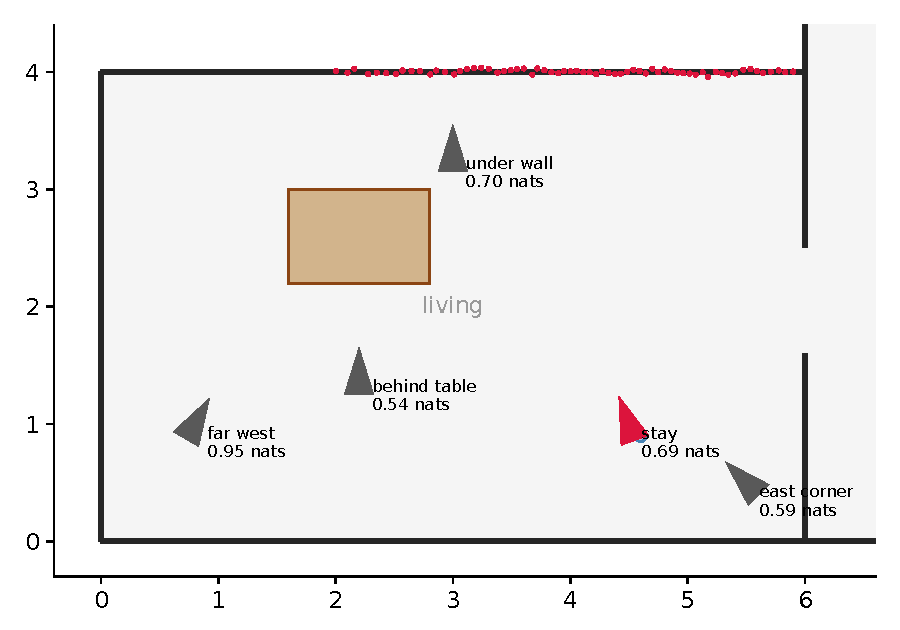
\includegraphics[width=\textwidth]{d1_candidates.pdf}
    \end{column}
    \begin{column}{0.4\textwidth}
      \small
      The robot (red) has seen the east part of the north wall. Five candidate viewpoints:
      \begin{itemize}
        \item ``far west'' sees the \emph{fewest} new points except one, yet gains the
              \emph{most}: it adds lever arm where the current information is weak;
        \item ``stay'' gains exactly $\ln 2$. Why?
      \end{itemize}
    \end{column}
  \end{columns}
\end{frame}

\begin{frame}{Diminishing returns, and a warning}
  \begin{columns}[c]
    \begin{column}{0.45\textwidth}
      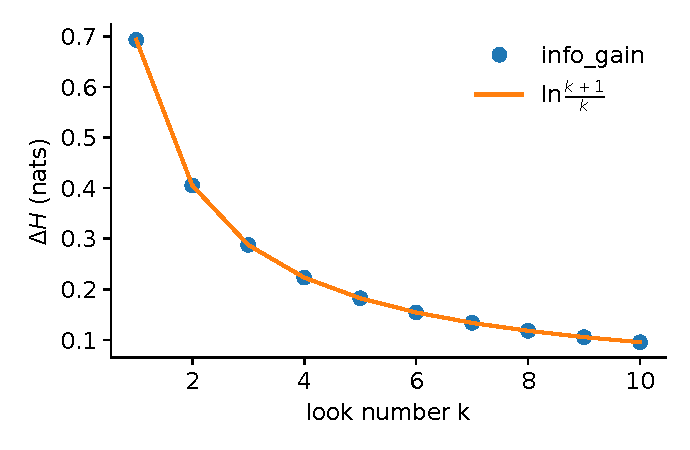
\includegraphics[width=\textwidth]{d1_diminishing.pdf}
    \end{column}
    \begin{column}{0.53\textwidth}
      \small
      The $k$-th identical look gives $|\,(k{+}1)\Lambda_1| / |\,k\Lambda_1|=((k{+}1)/k)^2$ for
      two parameters, so
      \[ \Delta H_k = \ln\frac{k+1}{k}. \]
      \pause
      \alert{But this assumes each look's errors are independent.} On a robot, repeated looks
      share the pose error, the mount error and the calibration error, and those do not average
      away.\\[0.4em]
      Tomorrow we put a number on how little a repeat look is really worth.
    \end{column}
  \end{columns}
\end{frame}

\begin{frame}{Pricing travel in the same currency}
  The simplest two-term expected free energy, the one that drives the robot's viewpoint selection:
  \[
    G(v) = \underbrace{\beta\,\lVert v - x\rVert}_{\text{cost of travel}}
         - \underbrace{\Delta H(v)}_{\text{information gain}}
  \]
  \begin{itemize}
    \item $\beta$ is an \emph{exchange rate}, in nats per metre, not a tuning knob between two
          incommensurable objectives.
    \item In the lab: above $\beta\approx0.07$ nats/m the robot stays put and scans again,
          because the (overvalued) $\ln 2$ is free.
    \item The full version sums agent-owned terms over a horizon. That is Day 5.
  \end{itemize}
  \src{introduction.tex l.244--253; action.tex}
\end{frame}

\begin{frame}{One objective across time scales}
  The gradient of a $T$-step expected free energy with respect to the current command splits as
  \[
    \nabla_{u_t} G_T(\pi)
      = \underbrace{\nabla_{u_t} G_{t+1}(u_t)}_{\text{what a reactive controller computes}}
      + \underbrace{\sum_{\tau=t+2}^{t+T}\nabla_{u_t} G_\tau(\pi)}_{\text{what planning adds}}
  \]
  \begin{itemize}
    \item Reactive control is the leading term of planning. They are not two systems.
    \item The relatives you know (planning-as-inference, MPC, MPPI) sit on this line. They differ in
          how many terms they keep and how they estimate them.
  \end{itemize}
  \src{active\_inference.tex l.431--510, l.557--579}
\end{frame}

% =================================================================================================
\section{What measurement said}
% =================================================================================================

\begin{frame}{Is the derived objective better than a good heuristic?}
  The room explorer, written in nats with no free weights, against the hand-tuned scorer it
  replaced. Both were run over the \textbf{same 594 real room layouts}, paired.
  \vspace{0.3em}
  \begin{center}\small
  \begin{tabular}{@{}l r r r@{}}
    \toprule
     & IoU mean & IoU median & Hausdorff median \\
    \midrule
    hand-tuned scorer & 0.9794 & 0.9880 & 0.038 m \\
    derived objective & 0.9806 & 0.9870 & 0.069 m \\
    \midrule
    paired difference & \multicolumn{3}{l}{$+0.0013\pm0.0030$; better / worse / tied $=238/298/58$, sign test $p=0.011$} \\
    \bottomrule
  \end{tabular}
  \end{center}
  \begin{itemize}\small
    \item It wins the mean and loses the count. Five rescued rooms carry the whole mean; without
          them the difference is $-0.00085$.
    \item The verdict is \alert{equivalence}, and the case for the derived form rests on its having
          no free parameters, not on performance.
  \end{itemize}
  \small On Day 5 we will see that even this IoU was not measuring what we thought it was.
  \src{experiments.tex l.1404--1446}
\end{frame}

\begin{frame}{Free energy is not computation}
  \begin{measured}{a better model does not save arithmetic}
    Injecting a body-model error from 0 to 10\%:
    \begin{itemize}
      \item the solver iterations per correction stay flat to within a twentieth;
      \item the size of the correction grows by about half as much again.
    \end{itemize}
  \end{measured}
  \begin{itemize}
    \item The agent pays in \emph{how far its beliefs must move}. The arithmetic doing the moving
          is nearly constant.
    \item ``A better model saves the agent work'' has to say \emph{which} work. The two readings
          come apart, and an endpoint chosen on the wrong reading measures nothing.
  \end{itemize}
  \src{active\_inference.tex l.835--848}
\end{frame}

\begin{frame}{Doing nothing can be an epistemic act}
  \begin{measured}{gyro bias, two legs of the same tour}
    The share of the bias posterior that came from data rather than from the prior: about
    \textbf{half} on one leg, \textbf{almost all} on the other. The only difference was that the
    robot happened to stand still for a few minutes.
  \end{measured}
  \begin{itemize}
    \item The bias regresses on elapsed time alone, so the action that teaches it is the one that
          only spends time: \alert{stopping}.
    \item The body is instrumented by everything the robot does, because every action passes
          through it. The world is sampled only where the robot looks.
    \item Hence: epistemic actions for rooms and objects, almost none for the body (Day 3).
  \end{itemize}
  \src{active\_inference.tex l.850--880, l.952--968}
\end{frame}

\begin{frame}{A factor inherits the errors of what it is estimated through}
  \begin{columns}[T]
    \begin{column}{0.52\textwidth}
      \begin{itemize}
        \item The body is learnt from the localiser's corrections, which are fitted against the
              room. So a wrong map is charged to the wheels.
        \item \alert{A robot in a room whose map is wrong will conclude that its wheels are
              wrong.}
        \item And it gets \emph{quieter}, not louder: once the body has absorbed the map's
              distortion, the two agree. The state is internally consistent and externally wrong.
      \end{itemize}
    \end{column}
    \begin{column}{0.45\textwidth}
      \begin{measured}{an omitted parameter}
        Admitting a camera-mount translation the data cannot support moves the reported pitch by
        \textbf{nine times} its stated interval. An interval speaks only about the parameters the
        model contains.
      \end{measured}
    \end{column}
  \end{columns}
  \lesson{Carry an external reference. Never trust only what the agent computes about itself.}
  \src{active\_inference.tex l.899--950}
\end{frame}

% =================================================================================================
\section{Lab}
% =================================================================================================

\begin{frame}{Lab 1: a wall as a belief, and where to look next}
  \texttt{labs/day1.ipynb}, about 75 minutes. Today the robot knows its pose and we cheat on which
  points are the wall's.
  \begin{enumerate}\small
    \item Write the wall's residual and Jacobian; fit it with \texttt{laplace}.
    \item \textbf{Honesty test}: 500 scans; predicted vs empirical $\sigma$. Find the 10\% and fix
          the likelihood.
    \item \textbf{Model choice}: Manhattan vs free, by $\Delta F$. Then tilt the wall.
    \item \textbf{Where to look}: $\Delta H$ for five viewpoints. Guess first, then compute.
    \item \textbf{Diminishing returns}: the $k$-th look against $\ln\frac{k+1}{k}$.
    \item \textbf{Price travel}: $G=\beta d-\Delta H$. Find the $\beta$ at which the robot stops
          moving. Then answer the day's key question: what does $\ln 2$ assume?
    \item Go and look: predicted vs realised entropy drop.
  \end{enumerate}
\end{frame}

\begin{frame}{Tomorrow}
  \begin{columns}[c]
    \begin{column}{0.55\textwidth}
      The robot loses both of today's cheats:
      \begin{itemize}
        \item it no longer knows its pose;
        \item it no longer knows which points belong to which wall.
      \end{itemize}
      One wall becomes a room, the pose becomes one more belief, and the two must be estimated
      \emph{together}.\\[0.5em]
      And we measure the common-mode ceiling: how little a thousand points can teach when they
      share one error.
    \end{column}
    \begin{column}{0.4\textwidth}
      \begin{block}{Reading for Day 2}\small
        Thesis chapters:
        \begin{itemize}
          \item \emph{Estimating the Layout of an Unknown Room}, \S\S 1--5;
          \item \emph{The Room Concept Agent}, \S\S ``What is estimated'' and ``The observation
                model''.
        \end{itemize}
      \end{block}
    \end{column}
  \end{columns}
\end{frame}

\end{document}
